\clearpage\section{Application Screenshots}
These six candidate-provided captures show sign-in, overall monitoring, event investigation, personal risk, and the AI workspace. Their displayed content is unchanged. Counts and scores belong to the captured demonstration state; they are not evaluation measurements.

\begin{figure}[!ht]\centering
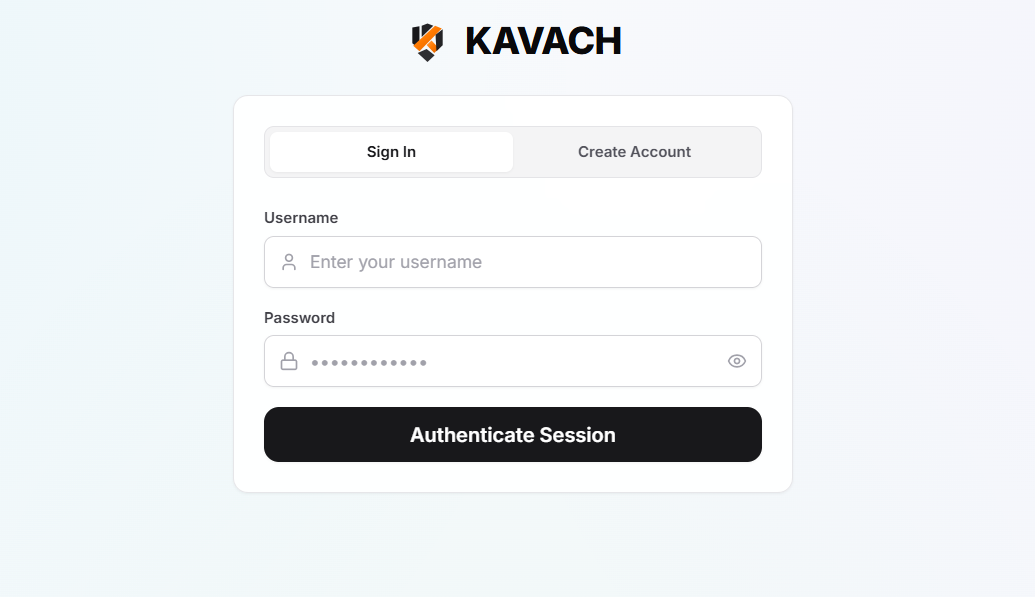
\includegraphics[width=.75\textwidth]{images/screenshot-login.png}
\caption{Sign-in interface with account-registration tab and authentication form.}\label{fig:screen-login}
\end{figure}

\begin{figure}[!ht]\centering
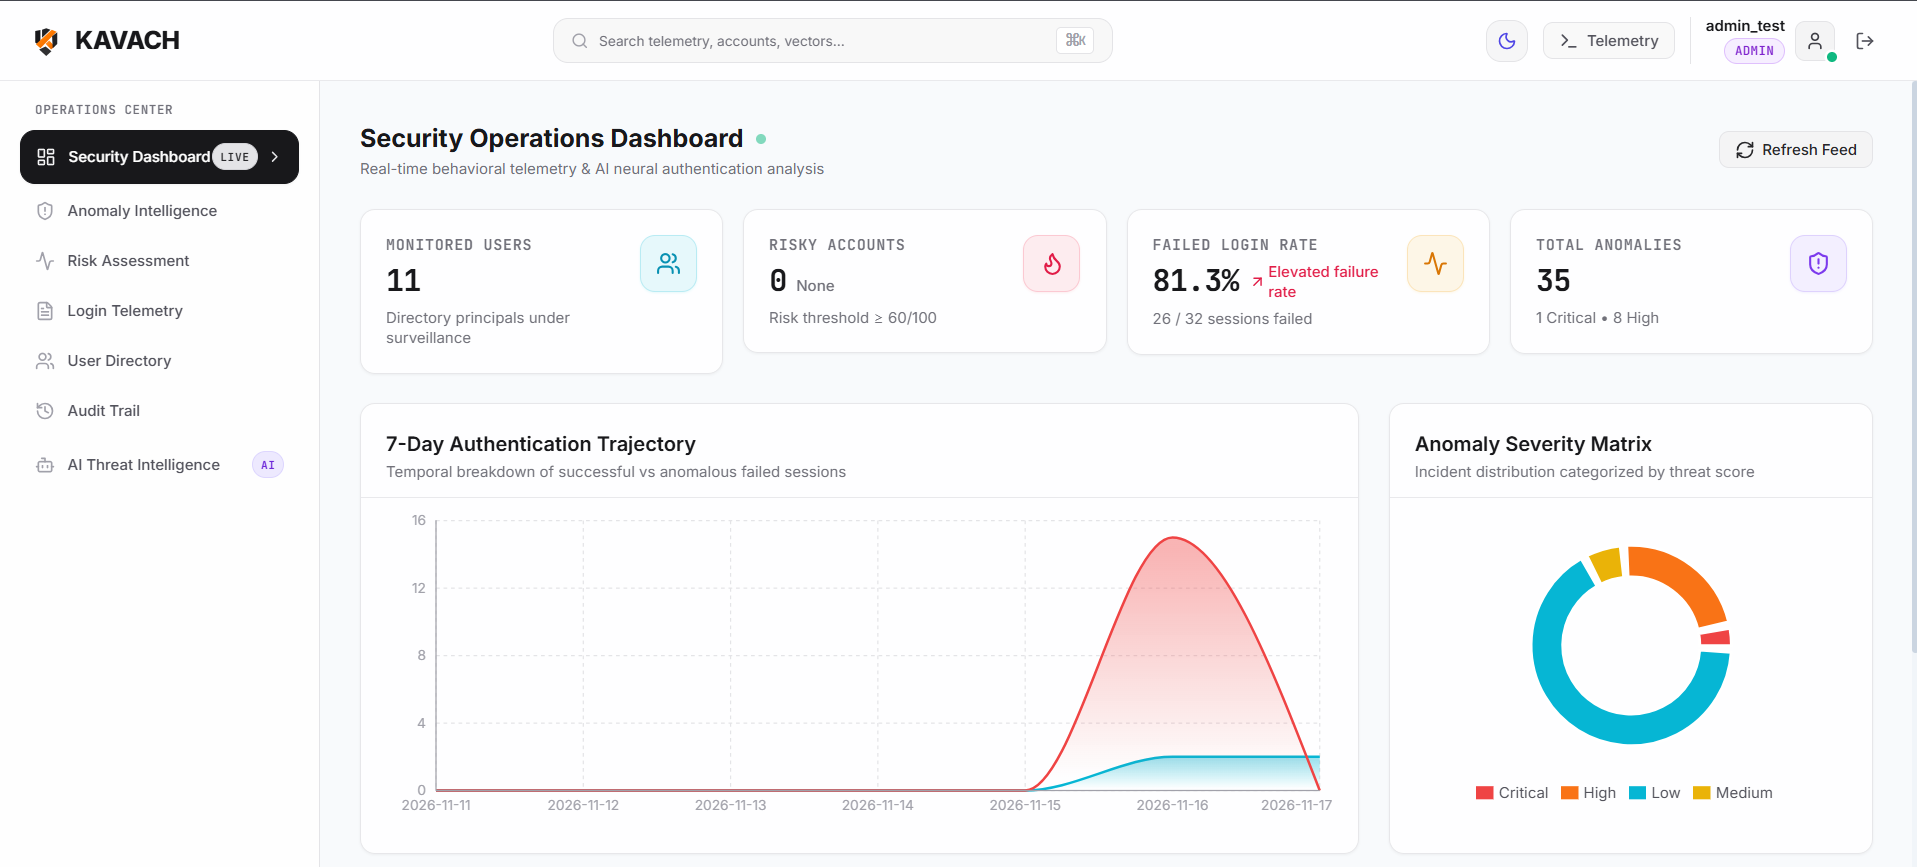
\includegraphics[width=\textwidth]{images/screenshot-dashboard.png}
\caption{Administrator dashboard: account counts, login outcomes, trend, and anomaly severity.}\label{fig:screen-dashboard}
\end{figure}

\clearpage\subsection{Anomaly Investigation and Login Telemetry}
The anomaly list shows matching rules and their alert weights. The login view provides the underlying event fields. Filters and action buttons are visible, but the captures do not show what happened after those actions were selected.

\begin{figure}[!ht]\centering
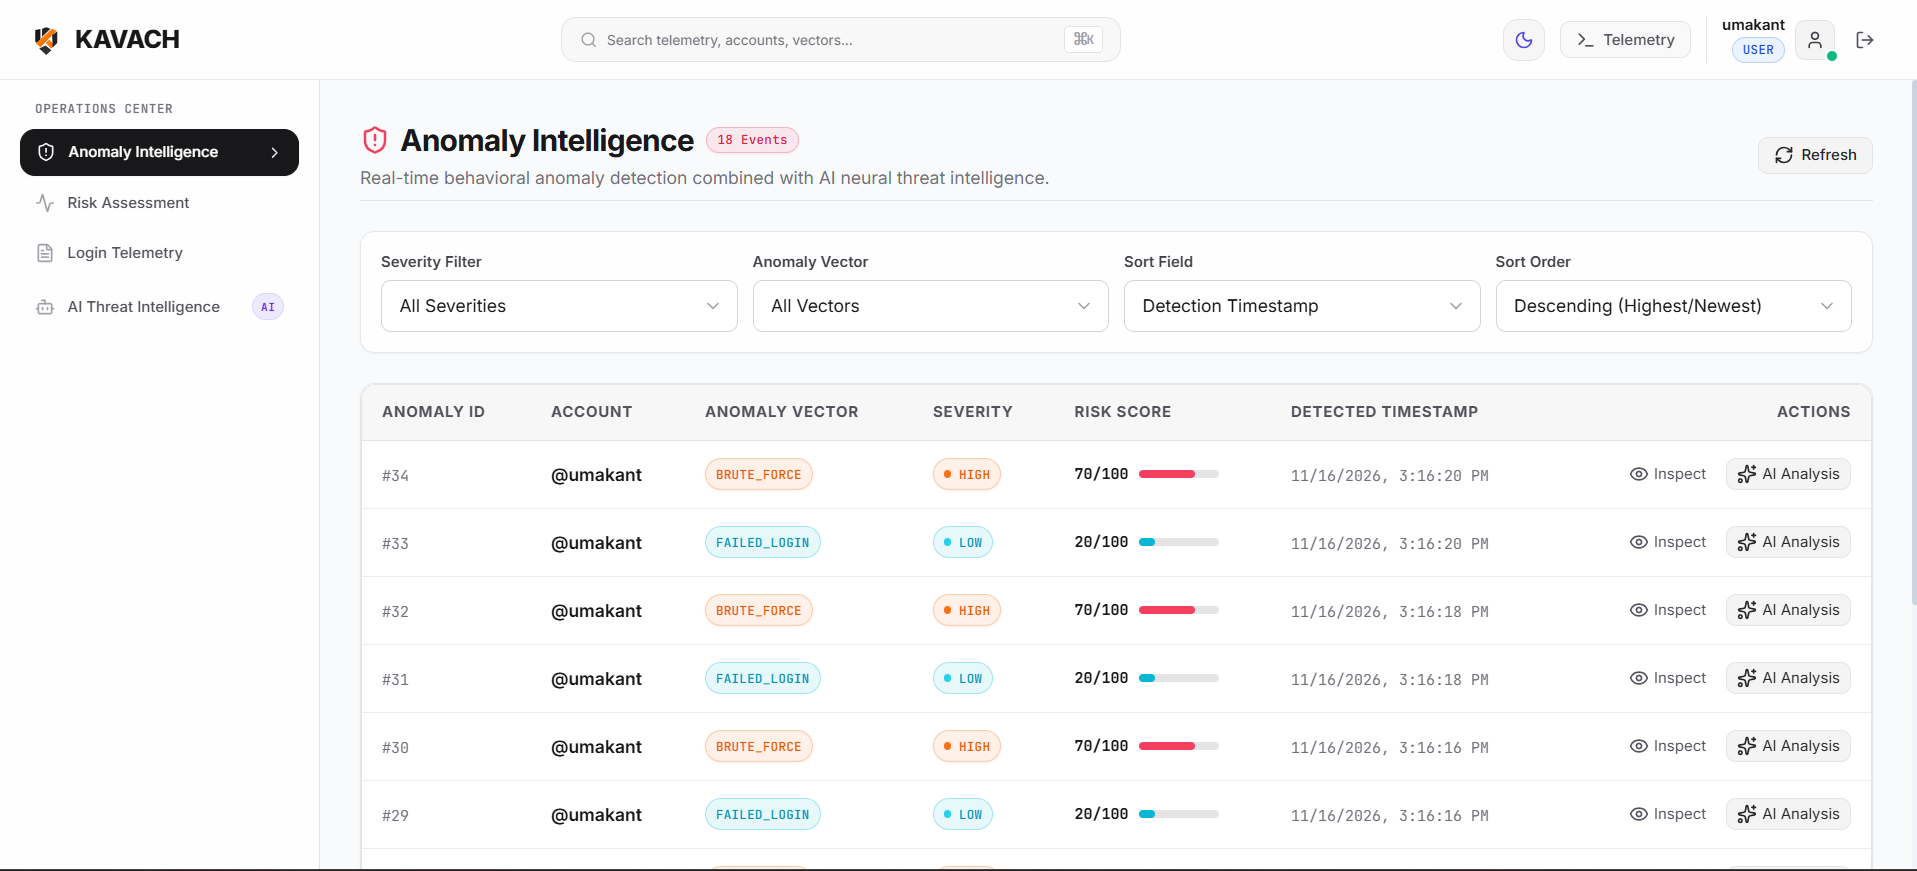
\includegraphics[width=\textwidth]{images/screenshot-anomalies.png}
\caption{User-scoped anomaly list with filters, rule types, severity, and alert weights.}\label{fig:screen-anomalies}
\end{figure}

\begin{figure}[!ht]\centering
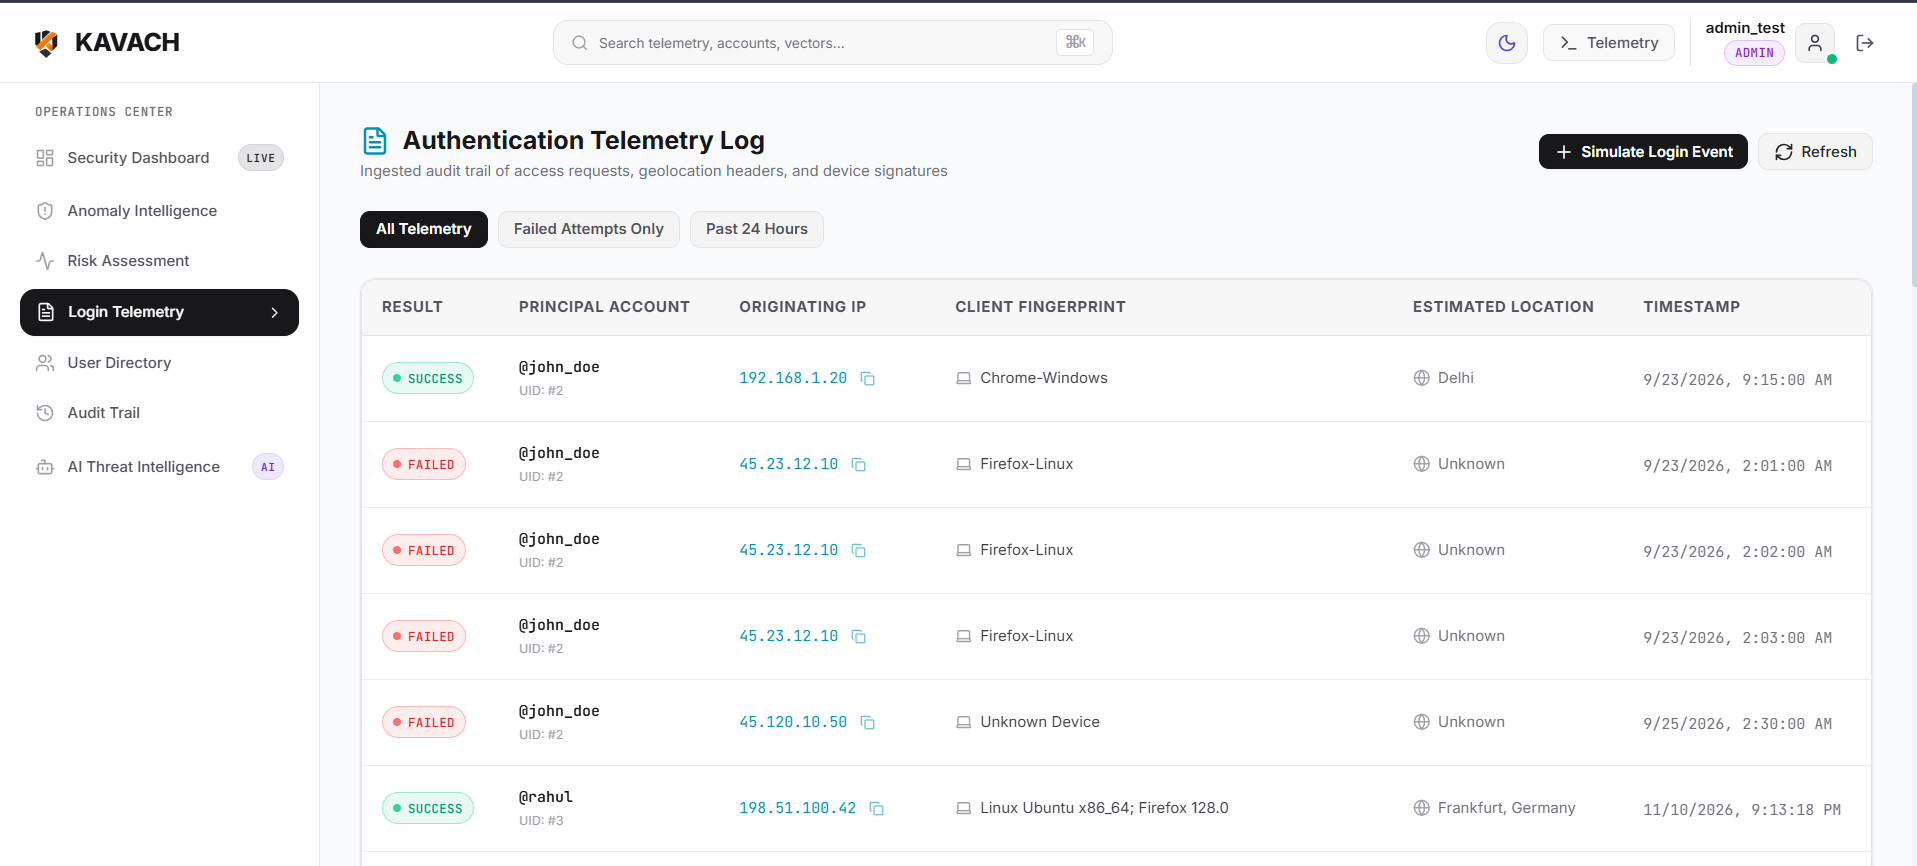
\includegraphics[width=\textwidth]{images/screenshot-telemetry.png}
\caption{Login telemetry showing successful and failed events with account and client metadata.}\label{fig:screen-telemetry}
\end{figure}

\clearpage\subsection{Personal Risk and AI Workspace}
The personal page shows the signed-in account's risk profile. Its recent 24-hour score and historical anomaly counts cover different periods. Although the interface uses subtitles such as ``Bayesian'' and ``neural'', Chapter 4 describes the implemented fixed rules and additive score. The AI screenshot captures the initial console before any completed model or tool execution.

\begin{figure}[!ht]\centering
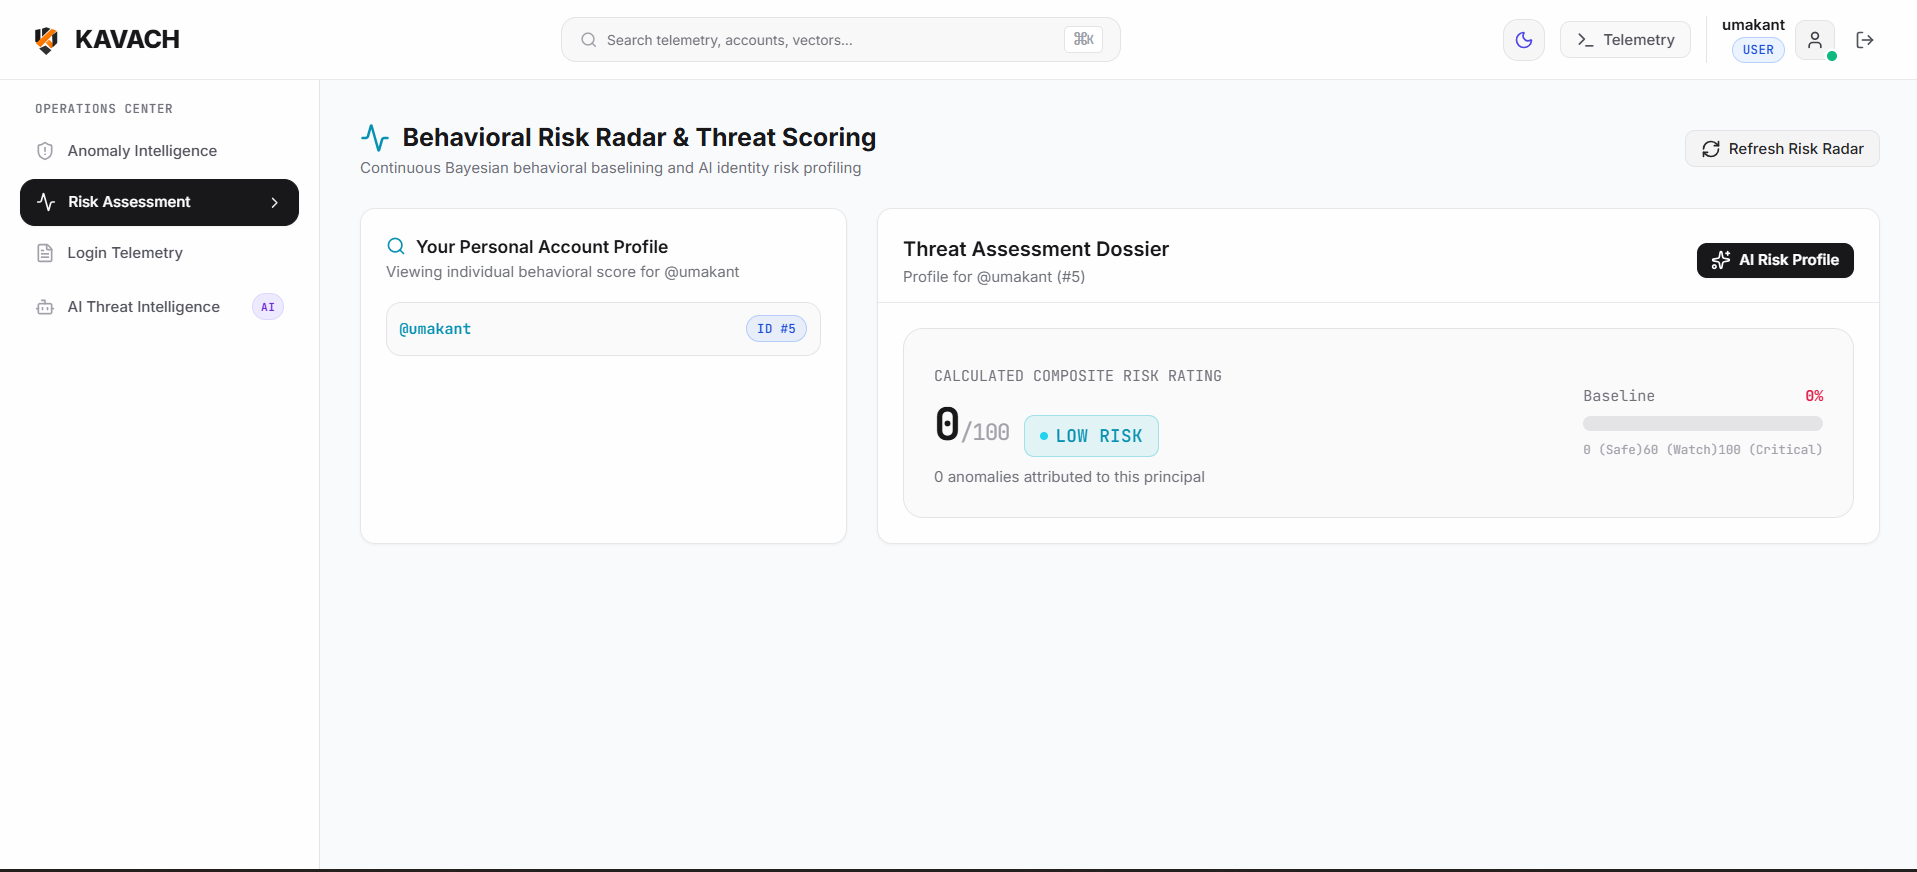
\includegraphics[width=\textwidth]{images/screenshot-personal-risk.png}
\caption{Personal risk view for the USER account, showing the displayed score and profile.}\label{fig:screen-risk}
\end{figure}

\begin{figure}[!ht]\centering
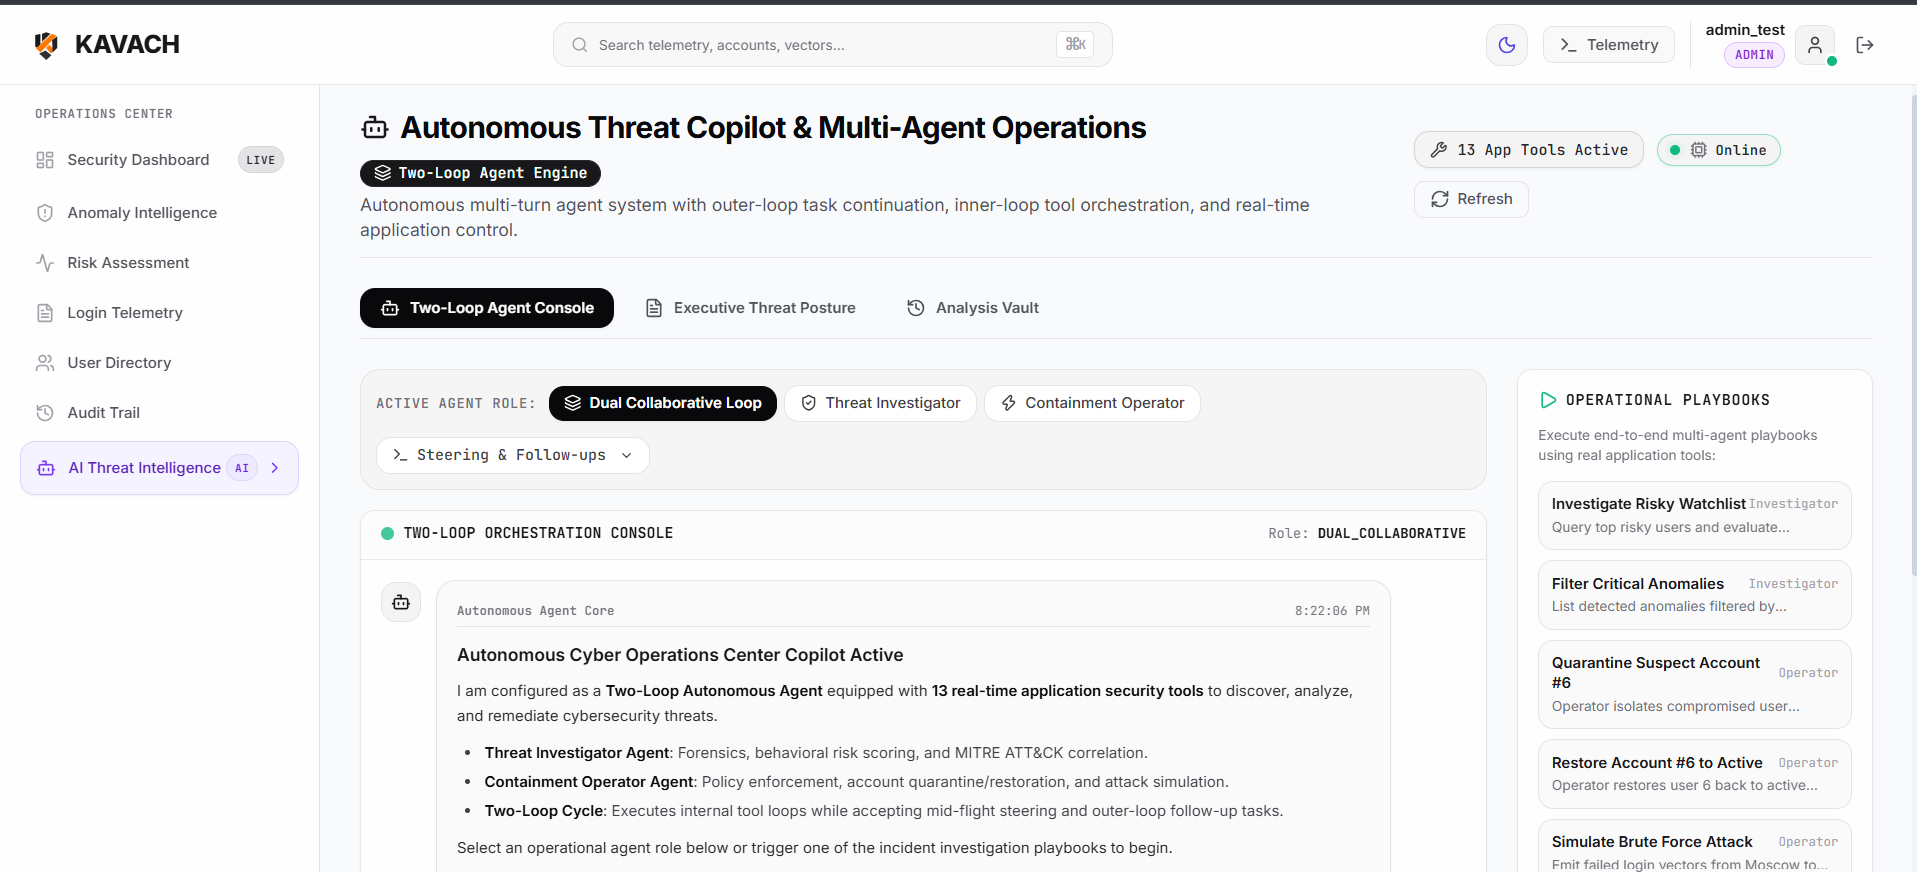
\includegraphics[width=\textwidth]{images/screenshot-ai-console.png}
\caption{AI workspace with agent-role selection, a 13-tool indicator, and operational playbooks.}\label{fig:screen-ai}
\end{figure}
